\documentclass[12pt, letterpaper]{umthesis}

%%%%%%%%%%%%%%%%%%%%%%%%%%%%%%%%%%%%%%%%%%%%%%%%%%%%%%%%%%%
%%%                  optional packages                  %%%
%%%%%%%%%%%%%%%%%%%%%%%%%%%%%%%%%%%%%%%%%%%%%%%%%%%%%%%%%%%
%% these packages are all optional. I include them here
%% because I use them, and I know they work with this class

\usepackage{sidecap} %put captions beside a figure
\usepackage{ifpdf} % check to see if compiling as dvi or pdf
\usepackage{rotating} % rotate some text
\usepackage{graphicx} % include graphics files
%\usepackage[all]{xy} %for making simple graphs
\usepackage{index} %this is newer and more fully featured than makeidx
\usepackage{hhline} %fancy rules
\usepackage{amsmath,amssymb} %extra math commands and symbols
\usepackage{mathptmx} %use times for normal text and math
\usepackage{helvet} %use helvetica font for sans-serif
\usepackage{courier} % use courier font for typewriter and fixed width
\usepackage{colortbl} %allows for color in tables
\usepackage{subfigure} % groups figures into one large one
\usepackage{longtable} % multi-page tables 
\usepackage{pdflscape} %better handling of landscape features
\usepackage{tabularx} %advanced tabular environment
\usepackage{multicol} % to use multiple columns
\usepackage{tikz} % package for making cool graphics - compatible with 
                  %  dvi, postscript, and pdf
\usetikzlibrary{arrows} % fancy arrows for tikz package
\usepackage{natbib} %more advanced handling of bibliographies
\bibpunct{(}{)}{;}{a}{,}{,} %settings for natbib, if using it
\usepackage[font=small,labelfont=bf,labelsep=quad]{caption} %more caption
\ifpdf %use these packages if we are compiling with pdf
  \usepackage{epstopdf} %automatically converts .eps files to .pdf
  \usepackage[final,expansion=true,protrusion=true]{microtype} 
    %advanced typesetting
\fi
%\usepackage[T1]{tipa} %phonetic fonts
%\usepackage{placeins} %prevent floats from floating past section
%\usepackage{flafter} %don't allow floats to appear before their definition
  %formatting
%\usepackage{chngpage}%this allows resetting margins within the document
%\usepackage[color]{showkeys}  % prints the names of labels that you use
                                 % handy for proofreading purposes
%\usepackage[dvips]{geometry} %tells dvips about paper size options
%\usepackage{svn} % to keep track of revisions
%\SVN $Author: robfelty $
%\SVN $Revision: 24 $
%\SVN $Date: 2007-05-10 15:13:37 -0400 (Thu, 10 May 2007) $
%\SVN $Id: example.tex 24 2007-05-10 19:13:37Z robfelty $
%\usepackage{timestamp} % to give me a timestamp

%%%%%%%%%%%%%%%%%%%%%%%%%%%%%%%%%%%%%%%%%%%%%%%%%%%%
%% sectsty allows to do some fancier formatting
%% of chapter and section titles - it is not clear
%% to me whether Rackham allows this or not
%%%%%%%%%%%%%%%%%%%%%%%%%%%%%%%%%%%%%%%%%%%%%%%%%%%

%\usepackage{sectsty}
%\makeatletter
%\chapternumberfont{%
%  \if@mainmatter%
%    \rule{\textwidth}{2pt}\\%
%    \vspace{-1em}\rule{\textwidth}{1pt}\\%
%  \fi%
%  \centering \huge \bf%
%}
%\chaptertitlefont{%
%  \if@mainmatter%
%    \vspace{-1em} \rule{\textwidth}{1pt}\\[.2em]%
%  \fi%
%  \centering \huge \bf%
%}
%\makeatother
%\usepackage[pdftex]{graphicx}

%%%%%%%%%%%%%%%%%%%%%%%%%%%%%%%%%%%%%%%%%%%%%%%%%%%%%%%%%%%
%%% fancy headers are not allowed by Rackham - however
%%% this does not mean that you can't use them for all other
%%% copies that you do not give to Rackham
%%%%%%%%%%%%%%%%%%%%%%%%%%%%%%%%%%%%%%%%%%%%%%%%%%%%%%%%%%%

%\usepackage{fancyhdr} 
%      \pagestyle{fancy} 
%      % with this we ensure that the chapter and section 
%      % headings are in lowercase. 
%      \renewcommand{\chaptermark}[1]{\markboth{#1}{}} 
%      \renewcommand{\sectionmark}[1]{\markright{\thesection\ #1}} 
%      \fancyhf{} % delete current setting for header and footer 
%      \fancyhead[LE,RO]{\thepage} 
%      \fancyhead[LO]{\rightmark} 
%      \fancyhead[RE]{\leftmark} 
%      %\fancyhead[RE,RO]{\bfseries\rightmark} 
%      %\fancyhead[LE,LO]{\bfseries\leftmark} 
%      %\fancyfoot[C]{\thepage}
%      \renewcommand{\headrulewidth}{0.5pt} 
%      \renewcommand{\footrulewidth}{0pt} 
%      \addtolength{\headheight}{0.5pt} % make space for the rule 
%      \fancypagestyle{plain}{% 
%      \fancyhead{} % get rid of headers on plain pages 
%      %\fancyfoot[C]{\thepage}
%      \fancyfoot{}
%      \renewcommand{\headrulewidth}{0pt} % and the line 
%      } 
\hfuzz2pt % Don't bother to report overfull hboxes if over-edge is < 2pt
\vfuzz2pt % Same for overfull vboxes (maybe just works for hfuzz?)  

%this command can be used for table headers that need to be rotated, thus the
%name rotth, for rotated table header -- it takes two arguments, the width of
%the parbox to create (which since it is rotated is more like height), and the
%text to put in it
\newcommand\rotth[2]{%
  \begin{sideways}%
    \parbox[b]{#1}{\raggedright #2}%
  \end{sideways}%
}
%this sets up a new command \dash, which makes nice dashes
\DeclareRobustCommand\dash{% 
\unskip\nobreak\thinspace\textemdash\thinspace\ignorespaces} 
   %in bookmarks, use regular dash instead of emdash
  \pdfstringdefDisableCommands{\renewcommand{\dash}{ - }} 

%%%%%%%%%%%%%%%%%%%%%%%%%%%%%%%%%%%%%%%%%%%%%%%%%%%%
%% additional options for the hyperref package (it is already loaded)
%%%%%%%%%%%%%%%%%%%%%%%%%%%%%%%%%%%%%%%%%%%%%%%%%%%%
%  \hypersetup{
%  colorlinks,
%  bookmarksnumbered,
%  bookmarkstype={toc},
%  bookmarksopen={true},
%  bookmarksopenlevel={1},
%  pdfstartview={FitH},
%  citecolor={blue},
%  %linkcolor={black},
%  %urlcolor={black},
%  pdfpagemode={UseOutlines},
%  breaklinks=true
%  } 

%the next two lines will prevent hyphenation in phonetic transcriptions
%\usepackage{hyphenat}
%\newcommand{\ipa}[1]{\nohyphens{\textipa{#1}}}

%% redefine some rules for nice table formatting
\setlength{\arrayrulewidth}{.6pt}
\setlength{\doublerulesep}{0pt}

%% allow more floats on a page, and change the float separation from text
\setlength{\floatsep}{5pt}
\setlength{\intextsep}{5pt}
\renewcommand\floatpagefraction{.70}
\renewcommand\topfraction{.95}
\renewcommand\bottomfraction{.95}
\renewcommand\textfraction{.1}

%%%%%%%%%%%%%%%%%%%%%%%%%%%%%%%%%%%%%%%%%%%%%%%%%%%%%%%%%%%
%%                    line spacing                      %%%
%% Rackham requires onehalf or double spacing
%% The default for the class is onehalf
%% To change it for non-final copies, use one of the following options
%\singlespacing
%\doublespacing
%% The class file automatically singles spaces stuff which should
%% be single spaced according to rackham, like the bibliography,
%% titles, long quotations and such
%% However, if you want to, you can also change spacing for 
%% a portion of text like so:
%%\begin{singlespacing} ... \end{singlespacing}
%%%%%%%%%%%%%%%%%%%%%%%%%%%%%%%%%%%%%%%%%%%%%%%%%%%%%%%%%%%

%%%%%%%%%%%%%%%%%%%%%%%%%%%%%%%%%%%%%%%%%%%%%%%%%%%%%%%%%%%
%%%               title and author info                %%%%
%%%%%%%%%%%%%%%%%%%%%%%%%%%%%%%%%%%%%%%%%%%%%%%%%%%%%%%%%%%
\author{\LaTeX}
\program{Professional Typesetting}
\degree{Doctor of Philosophy}
% if you only have chair, use \chaircommitteemember
% if you have outside members, you can specify their institution in the
% optional argument 
\cochaircommitteemember{John Smith}{Professor}
\cochaircommitteemember{Mary Johnson}{Assistant Professor}
\committeemember[University of Hard Knocks]{Robert Hughes}{Professor}
\committeemember{Emily Dickens}{Assistant Professor}
\title{The most Rackham-standards compliant dissertation ever}

\makeindex %if you are including an index
%%%%%%%%%%%%%%%%%%%%%%%%%%%%%%%%%%%%%%%%%%%%%%%%%%%%%%%%%%%%%%%%%
%% IMPORTANT - learn to use includeonly - it is very helpful
%% 1. put each chapter in a separate file
%% 2. type \include{file} where you want it to go
%% 3. First you have to compile once with everything included, 
%%    then you can include only certain parts
%%
%% and the table of contents will still list all parts, 
%% the chapter numbers will still all be correct
%% and you can easily print out (or e-mail or whatever) just one chapter
%% if you like, you can even leave out all the frontmatter stuff by putting
%% it in a separate file as well
%%%%%%%%%%%%%%%%%%%%%%%%%%%%%%%%%%%%%%%%%%%%%%%%%%%%%%%%%%%%%%%%%
\includeonly{%
intro,%
exp1,%
exp2,%
exp3,%
conclusion,%
appendix
}
\begin{document}
%%%%%%%%%%%%%%%%%%%%%%%%%%%%%%%%%%%%%%%%%%%%%%%%%%%%%%%%%%%%%%%%%%%%
%% IMPORTANT -- must issue frontmatter, mainmatter, and backmatter
%% commands in right place. These commands handle page numbering and
%%  formatting of various parts
%% \frontmatter - right after begin document
%% \mainmatter - right before first chapter
%% \backmatter - right before bibliography
%%%%%%%%%%%%%%%%%%%%%%%%%%%%%%%%%%%%%%%%%%%%%%%%%%%%%%%%%%%%%%%%%%%%%
\frontmatter

%%%% these command change latex's default hyphenation a bit. 
% Setting tolerance low will encourage hyphenation. 
% Setting tolerance high will discourage hyphenation
\pretolerance=-1
\tolerance=1000
\adjdemerits=6400
\doublehyphendemerits=90000
\finalhyphendemerits=14400

\maketitle
%%%%% the finalabstract environment typesets the abstract as it should be
% for the copies that go to Rackham separate of the actual dissertation. 
\begin{finalabstract}
  your abstract here
\end{finalabstract}
\makecopyright

\begin{frontispiece}
  If we knew what we were doing, it wouldn't be called research\\
  \dash Albert Einstein
\end{frontispiece}

\begin{dedication}
  to Delores
\end{dedication}

\begin{acknowledgments}
  these people helped me
\end{acknowledgments}

\begin{preface}
  before reading this, you should know\dots
\end{preface}

\tableofcontents

% only use these commands if you have more than figure, table, and/or
% appendix, respectively
\listoftables
\listoffigures
\listofappendices

% the normal abstract is formatted the same as preface and acknowledgments,
% and is listed in the table of contents
\begin{abstract}
  your abstract here
\end{abstract}
\mainmatter
\chapter{The introduction}
Modern research on lexical access began in the 1950's (though
\cite{ColeRudnicky1983} note very similar research performed in the 1890's by
William Chandler Bagley).  Several statistical properties of the mental
lexicon have consistently been found to influence how humans process speech.
One of the earliest and most robust findings was that lexical frequency has a
strong influence on lexical access. Repeated research has shown that high
frequency words elicit quicker and more accurate responses than low
frequency words in a large variety of experimental conditions
(e.g.\ \cite{Broadbent1967, Taft1979, BenkiJASA}). Another factor which has
been reliably shown to affect lexical access is neighborhood density.
Neighborhood density is a metric of similarity, roughly defined as the degree
to which a word is similar to others (both phonological and orthographical
measures have been used). Words which have many similar words are said to be
in dense neighborhoods, whereas words which have few similar words are said to
be in sparse neighborhoods. In contrast to lexical frequency, which
facilitates the activation of a word in the brain, neighborhood density has
been found to inhibit activation (e.g.\ \cite{Luce1986, Luce1998, BenkiJASA,
Imai2005}). Of course these are not the only factors which affect language
processing, but they are the most frequently cited, and will be referred to
again in the following sections.
\begin{table*}[!htb]
  \centering
  \caption[Basic Predictions]{Basic Predictions: Predicted results are marked
  with a checkmark, and a relative effect size is also given.}
  \label{T:predictions}
  \begin{tabularx}{\textwidth}{%
    >{\setlength{\hsize}{1.5\hsize}\raggedright\arraybackslash}X%
    *{2}{>{\setlength{\hsize}{.7\hsize}\raggedright\arraybackslash}X}%
    *{2}{>{\setlength{\hsize}{1.05\hsize}\raggedright\arraybackslash}X}}
  \hline\hline
  \rule{0em}{1.1em}& English native listeners& German native listeners & 
       English non-native listeners & German non-native listeners\\[.3em]
  \cline{2-5}
  \rule{0em}{1.1em}lexical status & \checkmark robust& \checkmark
  robust& \checkmark less than native listeners& \checkmark less than native
  listeners\\
  morphology & marginal & more than English & less than L1& less than L1\\
  lexical frequency & \checkmark robust& \checkmark
  robust& \checkmark less than native listeners& \checkmark less than native
  listeners\\
  neighborhood density & \checkmark robust & \checkmark robust & \checkmark less
  than L1& \checkmark less than L1\\[.3em]
  \hline\hline
  \end{tabularx}
\end{table*}

\chapter{My first experiment}
\label{ch:firstExp}

This is my first experiment. I will try to prove the following things:
(Note that lists are single spaced, as Rackham wants, and that lists should
start a new paragraph, otherwise the single spacing will also apply to the
preceding paragraph).

\begin{itemize}
  \item lists are easy to use
  \item \LaTeX\ rocks
\end{itemize}

The following figure was drawn using the excellent pgf/tikz graphics package.
If you do not have this package, you should comment it out.

\begin{figure*}[htbp]
\centering
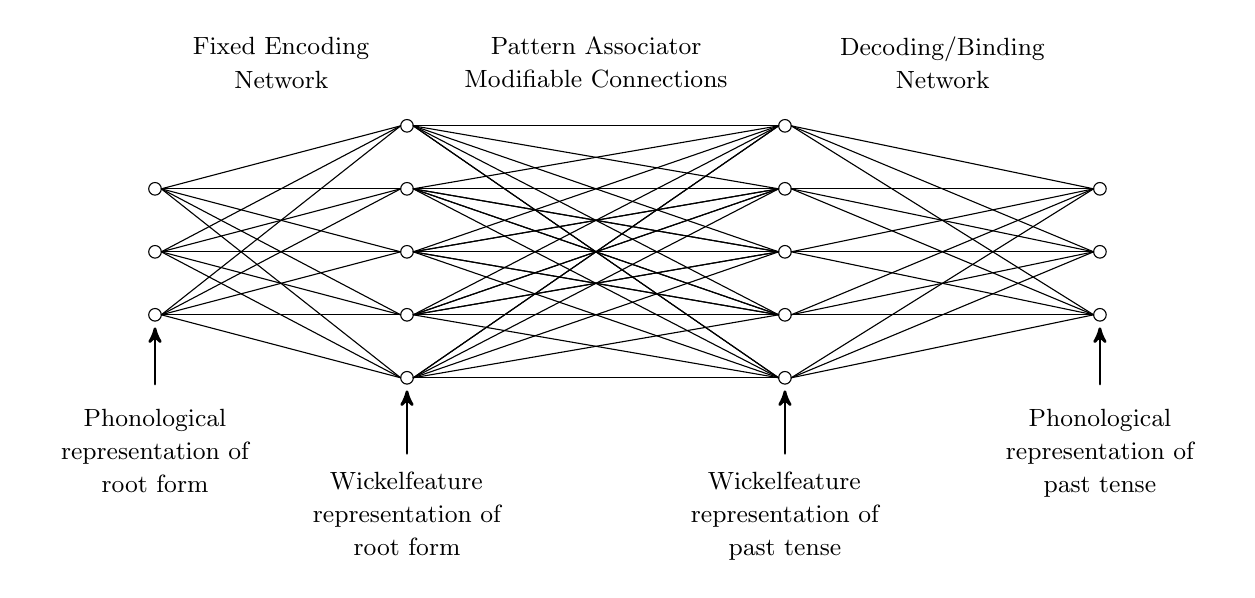
\begin{tikzpicture}[scale=.8,cap=round] 
% Styles 
\tikzstyle{information text}=[text badly centered]%, rounded corners,fill=red!10,inner sep=1ex] 
% The graphic 
\begin{scope}
\pgfsetarrowsend{stealth'} 
\pgfsetlinewidth{1pt} 
\draw (1,.9) -- (1,1.8)
  node[below=.9cm,text width=3cm,style=information text] 
  {\small Phonological representation of root form }; 
\draw (5,-.2) -- (5,.8)
  node[below=.9cm,text width=3cm, style=information text] 
  { \small Wickelfeature representation of root form }; 
\draw (11,-.2) -- (11,.8)
  node[below=.9cm,text width=3cm, style=information text] 
  { \small Wickelfeature representation of past tense }; 
\draw (16,0.9) -- (16,1.8)
  node[below=.9cm,text width=3cm, style=information text] 
  { \small Phonological representation of past tense }; 
\end{scope}
\draw (3,6)
  node[text width=3cm, style=information text] 
  { \small Fixed Encoding Network };
\draw (8,6)
  node[text width=4cm, style=information text] 
  { \small Pattern Associator Modifiable Connections };
\draw (13.5,6)
  node[text width=3cm, style=information text] 
  { \small Decoding/Binding Network };
% draw the nodes
\foreach \x in {1,16} 
  \foreach \y in {2,3,4} { 
    \draw (\x,\y) circle (0.1cm); 
  } 
\foreach \x in {5,11} 
  \foreach \y in {1,2,3,4,5} { 
    \draw (\x,\y) circle (0.1cm); 
  } 
% we add the lines for the nodes starting in y 2,3, and 4
\foreach \xa / \xb in {1.1 / 4.9, 5.1 / 10.9 , 10.9 / 5.1 , 15.9 / 11.1}
  \foreach \ya / \yb / \yc / \yd / \ye in {2 / 3 / 4 / 5 / 1, 3 / 4 / 5 / 1 /
  2, 4 / 5 / 1 / 2 / 3} {
  \draw (\xa,\ya) -- (\xb,\ya); 
  \draw (\xa,\ya) -- (\xb,\yb);
  \draw (\xa,\ya) -- (\xb,\yc); 
  \draw (\xa,\ya) -- (\xb,\yd); 
  \draw (\xa,\ya) -- (\xb,\ye); 
  }
% add remaining lines from y1 to y5
\foreach \xa / \xb in {5.1 / 10.9 , 10.9 / 5.1}
  \foreach \ya / \yb in {1 / 5, 5 / 1} {
  \draw (\xa,\ya) -- (\xb,\ya);
  \draw (\xa,\ya) -- (\xb,\yb);
  }
\end{tikzpicture} 

\caption[Model structure from \cite{Rumelhart1986}]{Model structure from
\cite{Rumelhart1986}}
\label{F:PDP}
\end{figure*}
The rest of this chapter proceeds as follows. Section \ref{sec:design}
describes the experiment design, while section~\ref{subsec:req} details the
requirements and section~\ref{subsubsec:setup} describes the experiment setup.
Section ~\ref{sec:method} describes my methods, while
section~\ref{subsec:procedures} gives details of the procedures and
section~\ref{subsubsec:firstSteps} goes over the first steps.

\section{Experiment design}
\label{sec:design}
I describe my first experiment in this section. 
\subsection{Experiment requirements}
\label{subsec:req}
Good design is expected.
\subsubsection{Experiment setup}
\label{subsubsec:setup}
The sound lab is needed.
\section{Method}
\label{sec:method}
I describe my methods in this section
\subsection{Procedures}
\label{subsec:procedures}
The following procedures were followed.
\subsubsection{First steps}
\label{subsubsec:firstSteps}
We carried out the experiment with the undergrads.


\chapter{My second experiment \dash which has a really long name, to
illustrate line breaking within the document as well as in the table of
contents}


\include{exp3}
\section{Conclusion and future work}
\label{sec:conclusion}

Current rule-based query optimizers do not provide a very intuitive and
conceptually streamlined framework to define rules and actions.  Our
experiences with the Volcano optimizer generator suggest that its model
of rules and the expression of these rules is much more complicated and
too low-level than it needs to be.  As a consequence, rule sets in
Volcano are fragile, hard to write, and debug.  Similar problems may
exist in other contemporary rule-based query optimizers.

We believe that rule-based query optimizers will be standard tools
of future database systems.  The pragmatic difficulties of using
existing rule-based optimizers led us to develop Prairie, an
extensible and structured algebraic framework for specifying rules.
Prairie is similar to existing optimizers in that it supports both
transformation rules and implementation rules.  However, Prairie
makes several improvements:
\begin{enumerate}
\item it offers a conceptually more streamlined model for rule specification;
\item rules are encapsulated, there are no ``hidden'' operators or
      ``hidden'' algorithms;
\item implementation hints (\eg enforcers) are deduced automatically;
\item and it has efficient implementations.
\end{enumerate}

We have explained how the first three points are important for
simplifying rule specifications and making rule sets less brittle for
extensibility.  A consequence is that Prairie rules are simpler and
more robust than rules of existing optimizers (\eg Volcano).  We
addressed the fourth point by building a P2V pre-processor which uses
sophisticated algorithms to compose and compact a Prairie rule set into
a Volcano rule set.  To demonstrate the scalability of our approach, we
rewrote the TI Open OODB rule set as a Prairie rule set, generated its
Volcano counterpart, and showed that the performance of the synthesized
Volcano rule set closely matches the hand-crafted Volcano rule set.

Our future work will concentrate on developing higher-level
abstractions using Prairie, including automatically generating Prairie
rule sets, and combining multiple Prairie rule sets to automatically
generate efficient optimizers.

\section*{Acknowledgments}
\label{sec:acknowledgments}

We wish to thank Texas Instruments, Inc.\ for making the Open OODB
source code available to us.  Comments by Jos\'e Blakeley, Anne Ngu,
Vivek Singhal, Thomas Woo and the anonymous referees greatly improved
the quality of the paper.

\appendix
% master: main
% format: latex

%%--------------------------------------------------------------------------
\begin{appendices}
%%--------------------------------------------------------------------------

%%--------------------------------------------------------------------------
\chapter{FIRST APPENDIX}
%%--------------------------------------------------------------------------

This is the 1st appendix.  Now alphabetic numbering starts for Appedices.
\ifAMS
\begin{equation}
    A=
    \begin{pmatrix}
	a_{11}&a_{12}&\ldots&a_{1n}\\
	a_{21}&a_{22}&\ldots&a_{2n}\\
	\vdots&\vdots&\ddots&\vdots\\
	a_{m1}&a_{m2}&\ldots&a_{mn}
    \end{pmatrix}
\end{equation}
\else
\begin{equation}
    A=
    \left(
    \begin{array}{cccc}
	a_{11}&a_{12}&\ldots&a_{1n}\\
	a_{21}&a_{22}&\ldots&a_{2n}\\
	\vdots&\vdots&\ddots&\vdots\\
	a_{m1}&a_{m2}&\ldots&a_{mn}
    \end{array}
    \right)
\end{equation}
\fi

%%--------------------------------------------------------------------------
\chapter{MATHEMATICAL SYMBOLS}
%%--------------------------------------------------------------------------
\label{sec:mathsym}

Here is the second appendix.  See how equations, figures, and tables in
appendices are numbered.
\ifAMS
\begin{equation}
    A=
    \begin{pmatrix}
	a_{11}&a_{12}&\ldots&a_{1n}\\
	a_{21}&a_{22}&\ldots&a_{2n}\\
	\vdots&\vdots&\ddots&\vdots\\
	a_{m1}&a_{m2}&\ldots&a_{mn}
    \end{pmatrix}
\end{equation}
\else
\begin{equation}
    A=
    \left(
    \begin{array}{cccc}
	a_{11}&a_{12}&\ldots&a_{1n}\\
	a_{21}&a_{22}&\ldots&a_{2n}\\
	\vdots&\vdots&\ddots&\vdots\\
	a_{m1}&a_{m2}&\ldots&a_{mn}
    \end{array}
    \right)
\end{equation}
\fi
%
\begin{eqnarray}
 \left(\int_{-\infty}^\infty e^{-x^2}\,dx\right)^2
 & =& \int_{-\infty}^\infty\int_{-\infty}^\infty
   e^{-(x^2+y^2)}\,dx\,dy \nonumber \\
 & =& \int_0^{2\pi}\int_0^\infty e^{-r^2}r\,dr\,d\theta \nonumber \\
 & =& \int_0^{2\pi}\left(\left. -\frac{e^{-r^2}}{2}
   \right|_{r=0}^{\infty}\,\right)\,d\theta \nonumber \\
 & =& \pi
\end{eqnarray}

otherwise

\begin{eqnarray}
\textstyle\sin18^\circ={\frac{1}{4}}(\sqrt5-1)\\
\ifAMS
x \in \mathbb{R} \\
\fi
k=1.38\times10^{-23}\rm\,J/^\circ K.
\end{eqnarray}

% Math-mode symbol & verbatim
\def\W#1#2{$#1{#2}$ &\ttfamily\string#1\string{#2\string}}
\def\X#1{$#1$ &\ttfamily\string#1}
\def\Y#1{$\big#1$ &\ttfamily\string#1}
\def\Z#1{\ttfamily\string#1}

%
\begin{table}
\caption{Greek Letters}\label{tab:greek}
\vspace{1ex}
\begin{tabular}{*8l}
\X\alpha	&\X\theta	&\X o		&\X\tau 	\\
\X\beta 	&\X\vartheta	&\X\pi		&\X\upsilon	\\
\X\gamma	&\X\iota	&\X\varpi	&\X\phi 	\\
\X\delta	&\X\kappa	&\X\rho 	&\X\varphi	\\
\X\epsilon	&\X\lambda	&\X\varrho	&\X\chi 	\\
\X\varepsilon	&\X\mu		&\X\sigma	&\X\psi 	\\
\X\zeta 	&\X\nu		&\X\varsigma	&\X\omega	\\
\X\eta		&\X\xi						\\
								\\
\X\Gamma	&\X\Lambda	&\X\Sigma	&\X\Psi 	\\
\X\Delta	&\X\Xi		&\X\Upsilon	&\X\Omega	\\
\X\Theta	&\X\Pi		&\X\Phi
\end{tabular}
\end{table}

\begin{table}
\caption{Binary Operation Symbols}\label{tab:bin}
\vspace{1ex}
\begin{tabular}{*8l}
\X\pm		&\X\cap 	&\X\diamond		&\X\oplus     \\
\X\mp		&\X\cup 	&\X\bigtriangleup	&\X\ominus    \\
\X\times	&\X\uplus	&\X\bigtriangledown	&\X\otimes    \\
\X\div		&\X\sqcap	&\X\triangleleft	&\X\oslash    \\
\X\ast		&\X\sqcup	&\X\triangleright	&\X\odot      \\
\X\star 	&\X\vee 	&\X\lhd$^*$		&\X\bigcirc   \\
\X\circ 	&\X\wedge	&\X\rhd$^*$		&\X\dagger    \\
\X\bullet	&\X\setminus	&\X\unlhd$^*$		&\X\ddagger   \\
\X\cdot 	&\X\wr		&\X\unrhd$^*$		&\X\amalg     \\
\X+		&\X-
\end{tabular}

$^*$ Not predefined in \LaTeXe.
     Use one of the packages  \textsf{latexsym}, \textsf{amsfonts} or
     \textsf{amssymb}.

\end{table}


\begin{table}
\caption{Relation Symbols}\label{tab:rel}
\vspace{1ex}
\begin{tabular}{*8l}
\X\leq		&\X\geq 	&\X\equiv	&\X\models	\\
\X\prec 	&\X\succ	&\X\sim 	&\X\perp	\\
\X\preceq	&\X\succeq	&\X\simeq	&\X\mid 	\\
\X\ll		&\X\gg		&\X\asymp	&\X\parallel	\\
\X\subset	&\X\supset	&\X\approx	&\X\bowtie	\\
\X\subseteq	&\X\supseteq	&\X\cong	&\X\Join$^*$	\\
\X\sqsubset$^*$ &\X\sqsupset$^*$&\X\neq 	&\X\smile	\\
\X\sqsubseteq	&\X\sqsupseteq	&\X\doteq	&\X\frown	\\
\X\in		&\X\ni		&\X\propto	&\X=		\\
\X\vdash	&\X\dashv	&\X<		&\X>		\\
\X:
\end{tabular}

$^*$ Not predefined in \LaTeXe.
     Use one of the packages  \textsf{latexsym}, \textsf{amsfonts} or
     \textsf{amssymb}.

\end{table}


\begin{table}
\caption{Punctuation Symbols}\label{tab:punct}
\vspace{1ex}
\begin{tabular}{*{5}{lp{3.2em}}}
\X,	&\X;	&\X\colon	&\X\ldotp	&\X\cdotp
\end{tabular}
\end{table}

\begin{table}
\caption{Arrow Symbols}\label{tab:arrow}
\vspace{1ex}
\begin{tabular}{*6l}
\X\leftarrow		&\X\longleftarrow	&\X\uparrow	\\
\X\Leftarrow		&\X\Longleftarrow	&\X\Uparrow	\\
\X\rightarrow		&\X\longrightarrow	&\X\downarrow	\\
\X\Rightarrow		&\X\Longrightarrow	&\X\Downarrow	\\
\X\leftrightarrow	&\X\longleftrightarrow	&\X\updownarrow \\
\X\Leftrightarrow	&\X\Longleftrightarrow	&\X\Updownarrow \\
\X\mapsto		&\X\longmapsto		&\X\nearrow	\\
\X\hookleftarrow	&\X\hookrightarrow	&\X\searrow	\\
\X\leftharpoonup	&\X\rightharpoonup	&\X\swarrow	\\
\X\leftharpoondown	&\X\rightharpoondown	&\X\nwarrow	\\
\X\rightleftharpoons	&\X\leadsto$^*$
\end{tabular}

$^*$ Not predefined in \LaTeXe.
     Use one of the packages  \textsf{latexsym}, \textsf{amsfonts} or
     \textsf{amssymb}.

\end{table}

\begin{table}
\caption{Miscellaneous Symbols}\label{tab:ord}
\vspace{1ex}
\begin{tabular}{*8l}
\X\ldots	&\X\cdots	&\X\vdots	&\X\ddots	\\
\X\aleph	&\X\prime	&\X\forall	&\X\infty	\\
\X\hbar 	&\X\emptyset	&\X\exists	&\X\Box$^*$	\\
\X\imath	&\X\nabla	&\X\neg 	&\X\Diamond$^*$ \\
\X\jmath	&\X\surd	&\X\flat	&\X\triangle	\\
\X\ell		&\X\top 	&\X\natural	&\X\clubsuit	\\
\X\wp		&\X\bot 	&\X\sharp	&\X\diamondsuit \\
\X\Re		&\X\|		&\X\backslash	&\X\heartsuit	\\
\X\Im		&\X\angle	&\X\partial	&\X\spadesuit	\\
\X\mho$^*$	&\X.		&\X|
\end{tabular}

$^*$ Not predefined in \LaTeXe.
     Use one of the packages  \textsf{latexsym}, \textsf{amsfonts} or
     \textsf{amssymb}.

\end{table}

\begin{table}
\caption{Variable-sized  Symbols}\label{tab:op}
\vspace{1ex}
\begin{tabular}{*6l}
\X\sum		&\X\bigcap	&\X\bigodot	\\
\X\prod 	&\X\bigcup	&\X\bigotimes	\\
\X\coprod	&\X\bigsqcup	&\X\bigoplus	\\
\X\int		&\X\bigvee	&\X\biguplus	\\
\X\oint 	&\X\bigwedge
\end{tabular}
\end{table}


\begin{table}
\caption{Log-like Symbols}\label{tab:log}
\vspace{1ex}
\begin{tabular}{*8l}
\Z\arccos &\Z\cos  &\Z\csc &\Z\exp &
	   \Z\ker    &\Z\limsup &\Z\min &\Z\sinh \\
\Z\arcsin &\Z\cosh &\Z\deg &\Z\gcd &
	   \Z\lg     &\Z\ln	&\Z\Pr	&\Z\sup  \\
\Z\arctan &\Z\cot  &\Z\det &\Z\hom &
	   \Z\lim    &\Z\log	&\Z\sec &\Z\tan  \\
\Z\arg	  &\Z\coth &\Z\dim &\Z\inf &
	   \Z\liminf &\Z\max	&\Z\sin &\Z\tanh
\end{tabular}
\end{table}


\begin{table}
\caption{Delimiters\label{tab:dels}}
\vspace{1ex}
\begin{tabular}{*8l}
\X(		&\X)		&\X\uparrow	&\X\Uparrow	\\
\X[		&\X]		&\X\downarrow	&\X\Downarrow	\\
\X\{		&\X\}		&\X\updownarrow &\X\Updownarrow \\
\X\lfloor	&\X\rfloor	&\X\lceil	&\X\rceil	\\
\X\langle	&\X\rangle	&\X/		&\X\backslash	\\
\X|		&\X\|
\end{tabular}
\end{table}

\begin{table}
\caption{Large Delimiters\label{tab:ldels}}
\vspace{1ex}
\begin{tabular}{*8l}
\Y\rmoustache&	\Y\lmoustache&	\Y\rgroup&	\Y\lgroup\\[5pt]
\Y\arrowvert&	\Y\Arrowvert&	\Y\bracevert
\end{tabular}
\end{table}

\begin{table}
\caption{Math mode accents}\label{tab:accent}
\vspace{1ex}
\begin{tabular}{*{10}l}
\W\hat{a}     &\W\acute{a}  &\W\bar{a}	  &\W\dot{a}	&\W\breve{a}\\
\W\check{a}   &\W\grave{a}  &\W\vec{a}	  &\W\ddot{a}	&\W\tilde{a}\\
\end{tabular}
\end{table}

\begin{table}
\caption{Some other constructions}\label{tab:other}
\vspace{1ex}
\begin{tabular}{*4l}
\W\widetilde{abc}	&\W\widehat{abc}			\\
\W\overleftarrow{abc}	&\W\overrightarrow{abc} 		\\
\W\overline{abc}	&\W\underline{abc}			\\
\W\overbrace{abc}	&\W\underbrace{abc}			\\[5pt]
\W\sqrt{abc}		&$\sqrt[n]{abc}$&\verb|\sqrt[n]{abc}|	\\
$f'$&\verb|f'|          &$\frac{abc}{xyz}$&\verb|\frac{abc}{xyz}|
\end{tabular}
\end{table}


%%--------------------------------------------------------------------------
\chapter{THIRD APPENDIX}
%%--------------------------------------------------------------------------

Here is the third appendix.
Watch the number of Figure \ref{fig:3} in this appendix.

\begin{figure}[h]
  \centering
  \unitlength 1in	    % make unit length to be 1 inch
  \begin{picture}(6,4)(0,0) % picture coordinates 6 in width, 4 in height,
			    % origin 0,0
    \put(1.4,2.6){\line(3,-1){3.0}} % draw a straight line at slope -1/3
				% starting at (1.4,2.6) of length 3.0
    \put(0,0){\vector(1,0){5.5}}
    \put(0,0){\vector(0,1){3}}
  \end{picture}
  \caption{A Picture Drawn with \LaTeX\ Commands}\label{fig:3}
\end{figure}

%%--------------------------------------------------------------------------
\end{appendices}
%%--------------------------------------------------------------------------



\backmatter
\bibliographystyle{mybibstyle} %my personal bibliography style
%\bibliographystyle{plain} %default bib style
\bibliography{felty}
%%%%%%%%%%%%%%%%%%%%%%%%%%%%%%%%%%%%%%%%%%%%%%%%%
%% if using an index, make sure to add it to the table of contents
%% and use phantomsection so hyperref links to the right page
%%%%%%%%%%%%%%%%%%%%%%%%%%%%%%%%%%%%%%%%%%%%%%%%%%%%%%%%%%%%
%\phantomsection %makes sure it points to the right page
%\addtocontents{toc}{chapter}{Index}
%\printindex
\end{document}
